% !TEX encoding = UTF-8
% !TEX TS-program = pdflatex
% !TEX root = ../tesi.tex
% !TEX spellcheck = it-IT

%**************************************************************
\chapter{Conclusioni}
\label{cap:conclusioni}
%**************************************************************

Questo capitolo finale espone le conclusioni tratte riguardo alle attività svolte durante il periodo di stage.

\section{Valutazione del risultato e di Ractive.js}
\begin{figure}[htp]
	\centering
	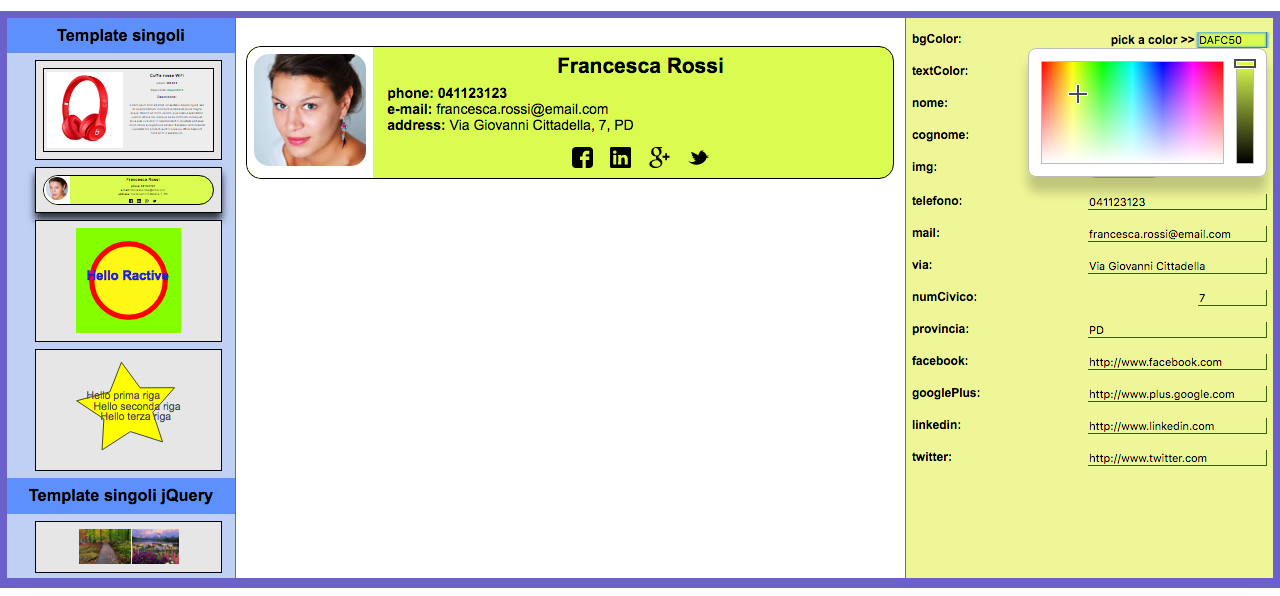
\includegraphics[scale=0.31]{../immagini/screenshot_app}
	\caption{Screenshot dell'applicazione realizzata.}
\end{figure}
I risultati ottenuti dallo studio delle librerie e l'applicazione realizzata soddisfano le aspettative dell'azienda.\\
La fase di prototipazione dei template, utilizzando la libreria \textit{Ractive.js}, ha messo in evidenza le potenzialità offerte da questo strumento e ha permesso all'azienda di trovare vari modi per sfruttare la libreria nello sviluppo dei loro prodotti.\\
Le richieste relative ai template sono state soddisfatte, dimostrando che è possibile creare template che si comportino in modo responsive e che integrino plug-in jQuery senza grandi sforzi da parte dello sviluppatore.\\
Inoltre è stata apprezzata la scelta di inserire il codice di attivazione per i plug-in jQuery all'interno della logica del template.\\
Per quanto riguarda i risultati ottenuti con l'applicazione, questi sono stati soddisfacenti per l'azienda, in quanto l'applicazione si comporta come era stato richiesto offrendo la possibilità di selezione e visualizzazione dei vari template e di modifica dei dati ad essi relativi.\\
Lo scopo principale dell'applicazione realizzata è stato quello di evidenziare le possibilità di integrazione della libreria \textit{Ractive.js} all'interno di una web application e di fornire un punto di partenza per lo sviluppo di un'eventuale estensione per l'applicativo aziendale \textit{Portal Studio}.
 
\subsection{Requisiti soddisfatti}
%RFF1.1.1 RFF2.1 RVF10
L'applicazione realizzata soddisfa tutti i requisiti obbligatori e desiderabili che sono stati individuati durante la fase di \textit{Analisi dei requisiti}.\\
Non sono stati soddisfatti i seguenti requisiti:
\begin{itemize}
	\item \textbf{RFF1.1.1} - La comparsa delle miniature all'interno della lista deve avvenire in modo animato;
	\item \textbf{RFF2.1} - La comparsa del template nel view-box deve avvenire in modo animato;
	\item \textbf{RVF10} - L'applicazione deve funzionare su \textit{Internet Explorer} versione 11.0 o superiore.
\end{itemize}
In totale sono stati soddisfatti 44 dei 46 requisiti funzionale e 9 dei 10 requisiti di vincolo.\\
Per quanto riguarda lo sviluppo dei template, il fatto che questi potessero essere resi responsive ed integrare plug-in jQuery possono essere considerati dei requisiti, anch'essi soddisfatti.
\section{Criticità}
L'unico problema riscontrato durante lo sviluppo dei template e dell'applicazione è quello relativo al caricamento \textit{on-demand} delle librerie jQuery.\\
Questo problema viene spiegato in dettaglio nella sezione \ref{subsec: problemi_lib}, esso è legato al funzionamento del \textit{browser} e alla mancanza di strumenti, offerti dallo standard, per controllare l'avvenuto caricamento delle librerie.\\
Un altro problema incontrato è relativo al comportamento del browser \textit{Internet Explorer}, che non visualizzava in maniera corretta i template SVG.\\
Questo fatto è risultato poco importante per l'azienda che considera \textit{Internet Explorer} ormai obsoleto dopo l'avvento di \textit{Microsoft Edge}.\\
Escludendo questi due problemi, non sono emersi altre criticità durante lo svolgimento del progetto.\\
I fattori che hanno portato a questo risultato sono sicuramente riconducibili al fatto che l'azienda mi ha dato molta autonomia durante il progetto e la difficoltà di quest'ultimo è risultata adeguata alla mia preparazione.
 
\section{Conoscenze acquisite}
Durante il periodo di stage sono state acquisite conoscenze sui \textit{template engine} e i loro possibili ambiti di utilizzo.\\
Le librerie analizzate durante il progetto erano sconosciute all'inizio dello stage, mentre a progetto terminato è stata ottenuta una discreta padronanza di esse ed in particolare della libreria \textit{Ractive.js} che, essendo stata utilizzata durante tutto il progetto, ha richiesto uno studio più approfondito.\\
Inoltre sono state affinate le conoscenze riguardanti i linguaggi per il web, in particolare JavaScript, che era già conosciuto prima dello stage, ma del quale erano sconosciuti vari aspetti come per esempio le \textit{promise}.\\
Sono state acquisite inoltre competenze sul tool di sviluppo proposto da \textit{Google}, su come utilizzare il debugger e come ottenere informazioni riguardanti i tempi di caricamento delle risorse e di rendering.\\
Lo stage ha reso possibile l'acquisizione di conoscenze relative all'ambito aziendale, dandomi la possibilità di osservare come vengono valutate le caratteristiche delle tecnologie che si ritengono promettenti per lo sviluppo di nuove soluzioni o per l'integrazione in quelle esistenti.\\
\'E stato inoltre possibile acquisire nozioni sull'organizzazione e sulle varie fasi del ciclo di vita del software, inoltre è stato possibile osservare le dinamiche aziendali e come si relaziona un team in ambito lavorativo.
